%************************************************
\chapter{Do PTAs observe inspiraling primordial black holes?} \label{chp:pbh}
%************************************************

%\vspace{1cm}
\begin{tcolorbox}[colframe=DESYcyan, colback=DESYcyan!10]
	\textbf{This chapter is based on the following publication:}
	\begin{itemize}[leftmargin=17pt]
		\item[\cite{Depta:2023qst}] \bibentry{Depta:2023qst}
	\end{itemize}
\end{tcolorbox}
\vspace{0.5cm}

\begin{flushright}
	\slshape
	Our hopes and expectations:\\
	Black holes and revelations\\ \medskip
	--- Starlight by \textsc{Muse}
\end{flushright}


\section{Introduction}

In chapter~\ref{chp:PTAs} we reviewed the recent \ac{PTA} results and concluded that the inspiral of \acp{SMBHB} is expected to contribute to \graffito{Astrophysical \acp{SMBHB} can only partially explain \ac{NANOGrav}} the observed \ac{GWB} at nHz frequencies~\cite{NANOGrav:2020bcs}. To match the observed signal amplitude, however, the local \ac{SMBHB} density would need to be an $\mathcal{O}(10)$ factor larger than previously
estimated~\cite{Casey-Clyde:2021xro,Kelley:2016gse, Kelley:2017lek}. Hence, the validity of this explanation is under active debate~\cite{Middleton:2020asl,Izquierdo-Villalba:2021prf,Curylo:2021pvf,Somalwar:2023bqv} and it is interesting to consider alternative sources.

In chapter~\ref{chp:ptabbn} we studied whether cosmological \acp{PT} could account for the novel \ac{PTA} signal. In the present chapter we move on and study the possibility that the observed \ac{GWB} could be due to inspiraling supermassive \textit{primordial} black holes. \graffito{Motivation for supermassive \acp{PBH}} The existence of \acp{PBH} in this mass range is motivated by yet unresolved puzzles concerning the observation of a large population of high-redshift quasars~\cite{Volonteri:2010wz, Volonteri:2021sfo, Shapiro:2004ud, Volonteri:2006ma, Tanaka:2008bv} and the related problem of missing seeds for non-linear structure formation at early times~\cite{Carr:2018rid, Hooper:2023nnl}.

To obtain the correct \ac{GWB} signal amplitude, however, we will find that a sizable abundance of \acp{PBH} is required, which is subject to strong constraints from \graffito{Our results contradict Atal et al.} various observational probes~\cite{Carr:2020gox}. It is therefore a non-trivial question whether inspiraling \acp{PBH} could constitute a viable explanation. Indeed we find, in accordance with ref.~\cite{Gouttenoire:2023nzr} which appeared shortly after our work~\cite{Depta:2023qst}, that it is \textit{not possible} to consistently explain the \ac{NANOGrav} data with homogeneously distributed \acp{PBH}. Specifically the parameter regions at very large \ac{PBH} masses which naively allow fitting the \ac{PTA} data (as done in~\cite{Atal:2020yic}) no longer result in a stochastic (or even continuous) signal. For clustered \acp{PBH}, on the other hand, we find that the formation of binary systems is more efficient and the merger rate is generally enhanced~\cite{Bringmann:2018mxj}, opening the possibility for an overall consistent description of the observed \ac{GWB}.

This chapter is structured as follows: We first review and extend the formalism required to compute the \ac{GWB} emitted from binary mergers for the case of clustered \acp{PBH} in section~\ref{sec:GWBfromPBH}. In section~\ref{sec:NPBH} we summarize our calculation of the number of \ac{PBH} binaries responsible for a given \ac{GWB}, justifying our claim \graffito{Outline of this chapter} that ref.~\cite{Atal:2020yic} came to an erroneous result. After discussing the relevant \ac{PBH} constraints and how to match the predicted signal to \ac{PTA} data in sections \ref{sec:PBHprod} and \ref{sec:PTAdatanalysis}, respectively, we present our results in section~\ref{sec:PBHresults}.



\section{Gravitational wave signal} \label{sec:GWBfromPBH}

We provided a first approximation for computing the \ac{GWB} spectrum from the inspiral of a population of \acp{SMBHB} in eq.~\eqref{eq:binaryGW}. Now, we will go beyond this: In the scenario at hand, the \ac{GWB} $h^2 \Omega_\gw (f)$ is generated from \ac{PBH} binary mergers occurring at a rate $R (t_\text{r})$ per comoving volume $V_\text{c}$ and cosmic \graffito{Going beyond $\Omega_{\mathrm{gw}}(f) \propto f^{2/3}$} time $t_\text{r}$. The frequencies accessible to \acp{PTA} can be well below the maximal frequency emitted during the merger and might therefore have been radiated long before coalescence, which we need to take into account. In particular, a given binary merging at time $t_{\text{r,merg}}$ has emitted a frequency $f_\text{r}$ in the cosmic rest frame, redshifted to a frequency $f = f_\text{r} / (1+z)$ today, at time $t_\text{r} = t_{\text{r,merg}} - \tau_{f_\text{r}}$, where
\begin{align}
	\tau_{f_\text{r}} = \frac{5 \times  2^{1/3}}{256 \, \pi^{8/3}} \, f_\text{r}^{-8/3} \, (G  m_\pbh)^{-5/3} \label{eq:tau_f_r}
\end{align}
is the time until coalescence for $f_\text{r}$~\cite{Maggiore:2007ulw}. As $t_{\text{r,merg}}$ is the argument for the \textit{merger} rate, the number of events per comoving volume and cosmic time emitting a frequency $f_\text{r}$ in the cosmic rest frame at cosmic time $t_\text{r}$ is given by $R (t_\text{r} + \tau_{f_\text{r}})$. Note that to the best of our knowledge this frequency-dependent rate has not been discussed in the literature concerning \acp{GW} generated by \acp{PBH} before. The \ac{GW} energy density parameter is given by (cf.~ref.~\cite{Phinney:2001di})
\begin{align}
	\Omega_\gw (f) = \frac{f}{\rho_\mathrm{crit}} \int_0^{t_0} \d t_\text{r} \left( R (t_\text{r} + \tau_{f_\text{r}}) \frac{\d E_\gw^\text{r}}{\d f_\text{r}} \right)_{f_\text{r} = (1+z) f} \eqsp, \label{eq:omega_gw}
\end{align}
where $t_0$ is the current cosmic time, $f_\text{r} = (1+z) \,f$ is the frequency that needs to be emitted  at the redshift $z = z(t_\text{r})$ corresponding to $t_\text{r}$ to detect a frequency $f$ today, and the \ac{GW} spectrum can be estimated by power-laws for inspiral, merger, and ringdown~\cite{Ajith:2007kx}\footnote{In our calculations we include a cut-off at $f_\text{r}= 1/t_\text{r}$, since smaller frequencies cannot have completed even one complete orbit.}
\begin{align}
	\frac{\d E_\gw^\text{r}}{\d f_\text{r}} \simeq \frac{(\pi  G)^{2/3}   m_\pbh^{5/3}}{3 \times 2^{1/3} } \begin{cases}
		f_\text{r}^{-1/3} &f_\text{r} < f_1 \\
		\frac{f_\text{r}^{2/3}}{f_1} &f_1 \leq f_\text{r} < f_2 \\
		\frac{f_\text{r}^2 f_4^4}{f_1 f_2^{4/3} [4 (f_\text{r} - f_2)^2 + f_4^2]^2} &f_2 \leq f_\text{r} < f_3 \\
		0  & f_3 \leq f_\text{r}\eqsp.
	\end{cases} \label{eq:gw_spectrum}
\end{align}
Here we assumed \acp{PBH} \graffito{\acp{GW} from inspiral, merger and ringdown}  with equal masses $m_\pbh$, $f_i = (a_i \eta^2 + b_i \eta + c_i) / (2 \pi G m_\pbh)$ with $\eta = 1/4$, and used the coefficients provided in Table~I of ref.~\cite{Ajith:2007kx}
\begin{subequations}
	\begin{align}
		(a_1, a_2, a_3, a_4) &= (2.97, 5.94 , 8.48, 5.08) \times 10^{-1}  \eqsp, \\
		(b_1, b_2, b_3, b_4) &= (4.48, 8.98, 12.8, 7.75) \times 10^{-2}  \eqsp, \\
		(c_1, c_2, c_3, c_4) &= (9.56, 19.1, 27.3, 2.24) \times 10^{-2}\eqsp. 
	\end{align}
\end{subequations}
Note that the \ac{GW} energy density $\Omega_{\gw}(f)$ is in fact a cosmological average of many \ac{PBH} binaries. We discuss the effect of only having access to a local realization of the \ac{GWB} within \ac{PTA} measurements in sec.~\ref{sec:NPBH}.

For the merger rate we adapt the calculation from ref.~\cite{Raidal:2017mfl}. We assume a monochromatic initial \ac{PBH} mass distribution, expecting that going to an extended distribution does not qualitatively change our results. A \ac{PBH} binary forms in the early Universe when the gravitational attraction between two neighboring \acp{PBH} overcomes the Hubble flow. A third close-by \ac{PBH} provides angular momentum such that the two \acp{PBH} do not simply collide~\cite{Nakamura:1997sm,Ioka:1998nz,Sasaki:2016jop}.

Clearly the merger rate depends on the local \ac{PBH} density at binary formation. It is therefore interesting to study the effect of clustering, which increases the global comoving number density $n_\pbh$ by the \graffito{Clustering $\delta_\mathrm{dc}$ increases the merger rate} local density contrast $\delta_\dc$. The density contrast can be considered constant on the scales relevant for binary formation~\cite{Raidal:2017mfl}. The comoving number density $n_\pbh$ can be expressed in terms of the \ac{PBH} mass $m_\pbh$, the fraction of \ac{PBH} \ac{DM} $f_\pbh$ and the \ac{DM} density $\rho_{\dm,0}$ today
\begin{align}
	n_\pbh = f_\pbh \, \frac{\rho_{\dm,0}}{m_\pbh}\eqsp.
\end{align}
The number density $\d n_3$ of the three-body configurations relevant for binary formation, where the comoving distance from a given \ac{PBH} in the binary to the other \ac{PBH} in the binary is within $x$ and $x+ \d x$ and the comoving distance to the third \ac{PBH} is within $y$ and $y + \d y$, is~\cite{Raidal:2017mfl}
\begin{align}
	\d n_3 (x, y) = \frac{n_\pbh}{2} \, \mathrm{e}^{-N_\pbh(y)} \, (4\pi  n_\pbh  \delta_\dc)^2 \, x^2 \, y^2 \, \d x \,  \d y \eqsp. \label{eq:pbh_n3}
\end{align}
Here, the factor of $1/2$ removes over-counting as either one of the \acp{PBH} in the binaries can be chosen and $\mathrm{e}^{-N(y)}$ makes sure that there is no fourth binary within the comoving distance $y$ (assuming Poisson statistics), where
\begin{align}
	N_\pbh (y) = \frac{4 \pi}{3} \, n_\pbh \, \delta_\dc \, y^3
\end{align}
is the expected number of binaries within a sphere of comoving distance $y$. The coalescence time $\tau$ of this binary is given by~\cite{Peters:1964zz,Raidal:2017mfl}
\begin{align}
	\tau (x, y) = \tilde{\tau} \left( \frac{x}{\tilde{x}} \right)^{37} \left( \frac{y}{\tilde{x}} \right)^{-21}\eqsp, 
\end{align}
where
\begin{align}
	\tilde{\tau} = \frac{3}{170} \frac{(a_\mathrm{eq}\tilde{x})^4}{(G m_\pbh)^3} \eqsp , && 
	\tilde{x} = \frac{3}{4 \pi} \frac{2  m_\pbh}{a_\mathrm{eq}^3 \, \rho_\mathrm{eq}}\eqsp,
\end{align}
$a_\mathrm{eq}$ and $\rho_\mathrm{eq}$ are the scale factor and total energy density at matter-radiation equality. The merger rate at time $t_\text{r}$ is then given by
\begin{align}
	R (t_\text{r}) &= \int_0^{\tilde{x}} \d x \, \int_x^\infty \d y \, \frac{\partial^2 n_3}{\partial x \, \partial y} \, \delta (t_\text{r} - \tau (x, y)) \nonumber \\
	&= \frac{9 \, \tilde{N}^{53/37}_\pbh}{296 \pi \, \delta_\dc \, \tilde{x}^3 \, \tilde{\tau}} \left( \frac{t_\text{r}}{\tilde{\tau}} \right)^{-34/37} \nonumber \\
	& \quad \times \left( \Gamma \left[ \frac{58}{37}, \tilde{N}_\pbh \left( \frac{t_\text{r}}{\tilde{\tau}} \right)^{3/16} \right] - \Gamma \left[ \frac{58}{37}, \tilde{N}_\pbh \left( \frac{t_\text{r}}{\tilde{\tau}} \right)^{-1/7} \right] \right)
\end{align}
with the incomplete gamma function $\Gamma$ and $\tilde{N}_\pbh = N_\pbh (\tilde{x})$. By substituting $t_\text{r} \rightarrow t_\text{r}+ \tau_{f_\text{r}}$ we can therefore compute the rate $R(t_\text{r} + \tau_{f_\text{r}})$ for the emission of this frequency $f_\text{r}$. Multiple merger steps, possibly present due to successive hierarchical merging of \ac{PBH} binaries with increasing mass due to large clustering, can be easily implemented by adding the rates and contributions to the \ac{GW} energy density parameter for the corresponding steps as detailed in ref.~\cite{Bringmann:2018mxj}. We include multiple merger steps when discussing the case of significant clustering, noting that this slightly shifts our results for $\delta_\dc = 10^3$ to lower \ac{PBH} abundances compared to only considering a single step.

\begin{figure}[t]
	\centering
	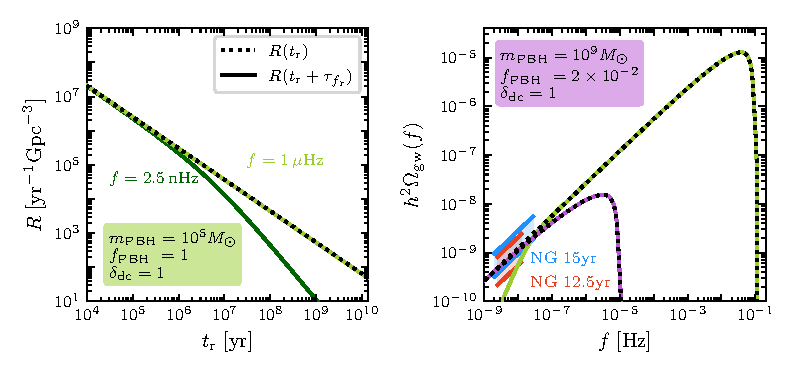
\includegraphics[width=\textwidth]{thesisplots/pbh/pbh_1.pdf}
	\caption{\textit{Left:} Rate for binaries merging at $t_\text{r}$ (dotted line) as well as rate for emitting \acp{GW} at $t_\text{r}$ with frequencies today $f = 1 \, \mu\mathrm{Hz}$ and $2.5 \, \mathrm{nHz}$ (solid light green and dark green lines) assuming $m_\pbh = 10^5 \, M_\odot$, $f_\pbh = 1$, and $\delta_\dc = 1$. \textit{Right:} \ac{GW} energy density $h^2\Omega_\text{gw}(f)$ obtained using the correct rate $R(t_\text{r} + \tau_{f_\text{r}})$ (solid lines) and instead using the merger rate $R(t_\text{r})$ in eq.~\eqref{eq:omega_gw} (dotted lines) for $m_\pbh = 10^5 \, M_\odot$, $f_\pbh = 1$, and $\delta_\dc = 1$ (green) and $m_\pbh = 10^9 \, M_\odot$, $f_\pbh = 2 \times 10^{-2}$, and $\delta_\dc = 1$ (purple). We also show the region where the \ac{NANOGrav} 12.5yr and 15yr signals are located assuming a power-law with slope $\gamma = 13/3$ (see eq.~\eqref{eq:13/3}).}
	\label{fig:rate_ogw}
\end{figure}


To illustrate the importance of the time when a given frequency is emitted we show in the left panel of fig.~\ref{fig:rate_ogw} the rate for binaries merging at $t_\text{r}$ (dotted blue line) with the \graffito{The correction $t_\mathrm{r} \rightarrow t_\mathrm{r} + \tau_{f_\mathrm{r}}$ is important!} one for \ac{GW} emission with frequencies $f = 1 \, \mu\mathrm{Hz}$ and $2.5 \, \mathrm{nHz}$ today (solid green and orange lines), assuming $m_\pbh = 10^5 \, M_\odot$, $f_\pbh = 1$, and $\delta_\dc = 1$ in each case. For instance, at $t_\text{r} = 10^8 \, \mathrm{yr}$ (i.e.\ $z \approx 30$) one obtains $\tau_{f_\text{r}}((1+z)1 \, \mu\mathrm{Hz}) \approx 130 \, \mathrm{yr}$ and $\tau_{f_\text{r}}((1+z)2.5 \, \mathrm{nHz}) \approx 1.1 \times 10^9 \, \mathrm{yr}$. Hence, the rate for the emission of \acp{GW} with the larger frequency (solid light green line) is very close to the merger rate (dotted line), whereas the rate for the emission of \acp{GW} with the smaller frequency (solid dark green line) differs significantly, i.e.~it takes the value that the dotted blue line attains $1.1 \times 10^9 \, \mathrm{yr}$ later.

In the right panel of fig.~\ref{fig:rate_ogw} we show $h^2 \Omega_\gw(f)$ as a function of the \ac{GW} frequency today according to eq.~\eqref{eq:omega_gw} (solid lines) as well as just inserting the merger rate $R (t_\text{r})$ instead of $R(t_\text{r} + \tau_{f_\text{r}})$ in the integral (dotted lines). The difference between those calculations is especially important for the low frequencies observed by \ac{NANOGrav} if the \ac{PBH} mass is relatively light.

We close the discussion of the \ac{GWB} signal by \graffito{Assumptions} mentioning some assumptions that entered in its calculation. These include
\begin{itemize}
	\item a monochromatic mass distribution for the \acp{PBH}~\cite{Raidal:2017mfl},
	\item a circular orbit of the \ac{PBH} binaries for the \ac{GWB} spectrum and the time until coalescence for a given frequency,
	\item neglecting the effect of other \acp{PBH} on the binaries~\cite{Ali-Haimoud:2017rtz,Raidal:2018bbj} as well as other environmental effects e.g.~due to accretion, and
	\item late-time formation of binaries~\cite{Raidal:2017mfl}.
\end{itemize}
Apart from the effect of other \acp{PBH} which can potentially significantly reduce their merger rate on binaries~\cite{Raidal:2018bbj}, these assumptions are not expected to have a qualitative impact on our results. A valuable test of these assumption is within reach using astrophysical $N$-body simulations, which are, however, computationally expensive and hence beyond the scope of this thesis.

\section{Expected number of binaries} \label{sec:NPBH}
The \ac{PTA} signals are reported as stochastic \acp{GWB}. While there \graffito{On the stochasticity of $\Omega_\mathrm{gw}$}  have been searches for signals of individual binaries in the data of different \acp{PTA}~\cite{IPTA:2023ero,Antoniadis:2023aac,NANOGrav:2023pdq}, no compelling evidence for these signals  was found. For sufficiently large \ac{PBH} masses and small abundances the expected signal will in general no longer resemble a stochastic background, as only very few binaries will contribute to the signal, causing inconsistency with observations.

The problem is exacerbated by the question of how well an actual distribution of merging binaries observed by a \ac{PTA} (corresponding to a local\footnote{Local on the scales relevant for a \ac{GW} signal in \ac{PTA} observations, i.e.\ at least within a sphere around earth with a few light-years radius such that correlations between different pulsars can be affected.} value of \Ac{GW} energy density $\Omega_{\gw, \mathrm{loc}}$) would reproduce the global average of the \ac{GW} energy density $h^2 \Omega_\gw (f) = h^2 \langle \Omega_{\gw, \mathrm{loc}} (f) \rangle$, i.e.\ how well the global mean is reproduced by the binaries that are in our past light cone. As shown in ref.~\cite{Ellis:2023owy}, even relatively generic distributions of binary \graffito{Good predictions require large $\bar{N}$} mergers, scaling with the luminosity distance squared, can lead to wide distributions in $\Omega_{\gw, \mathrm{loc}}$, with width-to-mean ratios scaling like $\Delta \Omega_{\gw, \mathrm{loc}} / \Omega_\gw \propto  \bar{N}^{-1/3}$ with $\bar{N}$ the expected number of binaries contributing to a certain frequency range, slower than predicted from the central limit theorem $\propto \bar{N}^{-1/2}$.

To calculate the average number of binaries contributing to a certain frequency range, recall that $R(t_\text{r} + \tau_{f_\text{r}})$ is the number of binaries per comoving volume $V_\text{c}$ and per time \graffito{On calculating $\bar{N}$} interval in the cosmic rest frame $t_\text{r}$ emitting with a frequency $f_\text{r}$. Hence, the number of binaries $\d \bar{N}$ emitting at redshifts between $z$ and $z + \d z$ with a frequency within the logarithmic interval $\d \ln f_\text{r}$ around $f_\text{r}$ is~\cite{Sesana:2008mz}
\begin{align}
	R (t_\text{r}+ \tau_{f_\text{r}}) &= \frac{\d^2 \bar{N}}{\d t_\text{r} \, \d  V_\text{c}}  = \frac{\d z}{\d t_\text{r}} \frac{\d^2 \bar{N}}{\d z \, \d \ln f_\text{r}} \frac{\d \ln f_\text{r}}{\d t_\text{r}} \frac{\d t_\text{r}}{\d z} \frac{\d z}{\d V_\text{c}} \nonumber \\
	&= \frac{\d^2 \bar{N}}{\d z \, \d \ln f_\text{r}} \left( - \frac{\d \ln f_\text{r}}{\d \tau_{f_\text{r}}} \right) \frac{\d z}{\d V_\text{c}}\eqsp,
\end{align}
where we used that the time in the cosmic rest frame a source is emitting within the frequency interval is given by
\begin{align}
	\d t_\text{r} \frac{\d \ln f_\text{r}}{\d t_\text{r}} = - \d t_\text{r} \frac{\d \ln f_\text{r}}{\d \tau_{f_\text{r}}} \,,
\end{align}
as $\tau_{f_\text{r}}$ is the time until coalescence for $f_\text{r}$. Since the binaries emitting in the logarithmic frequency interval $\d \ln f_\text{r}$ around $f_\text{r}$ are detected today in a logarithmic frequency interval $\d \ln f$ around $f$, where $\d \ln f_\text{r} = \d f_\text{r} / f_\text{r} = \d f / f = \d \ln f$, we have
\begin{align}
	\frac{\d^2 \bar{N}}{\d z \, \d \ln f} = \frac{\d^2 \bar{N}}{\d z \, \d \ln f_\text{r}} \;.
\end{align}
With eq.~\eqref{eq:tau_f_r} and the definition of the comoving volume in a spatially flat universe
\begin{align}
	V_\text{c} (z) = \frac{4 \pi}{3} [d_\text{c}(z)]^3 = \frac{4 \pi}{3} \left( \int_0^z \frac{\d z'}{H(z')} \right)^3 \eqsp ,
\end{align}
where $d_\text{c}$ is the comoving distance and $H$ is the Hubble rate, we find
\begin{align}
	\frac{\d^2 \bar{N}}{\d z \, \d \ln f} = \frac{8}{3} \, \tau_{f_\text{r}} \, \frac{4 \pi \, [d_\text{c}(z)]^2}{H(z)} \, R (t_\text{r}(z) - \tau_{f_\text{r}})\eqsp.
\end{align}
The average number of binaries $\bar{N} (f_-, f_+)$ contributing to \acp{GW} of frequencies between $f_-$ and $f_+$ is therefore given by\footnote{The \textit{actual} number of binaries is then Poisson distributed with mean $\bar{N} (f_-, f_+)$.}
\begin{align}
	\bar{N} (f_-, f_+) = \int_{f_-}^{f_+} \frac{\d f}{f} \, \int_0^\infty \d z \, \frac{8}{3} \, \tau_{f_\text{r}} \frac{4 \pi \, [d_c(z)]^2}{H(z)} \, R (t_\text{r}(z) - \tau_{f_\text{r}})\eqsp.
\end{align}
As we are interested in the number of binaries contributing to the \ac{NANOGrav} 15yr signal, we take the frequency interval to span over the corresponding lowest 14 Fourier modes, i.e.~$f_- = 1/T_\text{obs}^\text{15yr} = 1.98 \, \text{nHz}$ and $f_+ = 14/T_\text{obs}^\text{15yr} = 27.7 \, \text{nHz}$, cf.~fig.~\ref{fig:observability}.

The signal prediction for \acp{PTA} is crucially affected by the expected number of binaries emitting in the relevant frequency band~\cite{Ellis:2023owy}. Generally, the local \ac{GWB} $h^2 \Omega_{\gw, \mathrm{loc}} (f)$ that may be observed by a \ac{PTA} is obtained by adding individual PBH binaries (the total number drawn from a Poisson distribution with mean $\bar{N} (f_-, f_+)$) distributed according to $\d^2 \bar{N} / (\d z \, \d \ln f)$. In particular, $h^2 \Omega_{\gw, \mathrm{loc}}(f)$ is \textit{not} deterministic given model parameters (mass, abundance, and clustering of \acp{PBH}), but instead stochastic in itself. The statistics of $h^2 \Omega_{\gw, \mathrm{loc}}(f)$ can be evaluated using Markov chain Monte Carlo methods or moment generating functions~\cite{Ellis:2023owy}. Due to the considerable additional numerical effort we leave this for future studies, use the global average signal prediction $h^2 \Omega_\gw (f)$, and identify regions in parameter space where we \graffito{High signal prediction uncertainty for $\bar{N} \sim \mathcal{O}(\mathrm{few})$} expect a significant deviation from the global average. If $\bar{N} (f_-, f_+) \gg 1$, a lot of different PBH binaries contribute to the \ac{GW} signal and the local \ac{GWB} $h^2 \Omega_{\gw, \mathrm{loc}} (f)$ is close to the global average $h^2 \Omega_\gw (f)$. This holds even though uncertainties due to some close-by binaries can be relevant for $\bar{N} (f_-, f_+) \lesssim 100$~\cite{Ellis:2023owy}. If $\bar{N} (f_-, f_+) \sim \mathcal{O} (\mathrm{few})$, i.e.~if the \ac{GW} signal is composed of only a few binaries, the uncertainty in the signal prediction is considerable. Arguably, it would be more appropriate to search for individual \ac{GW} events instead of a \ac{GWB}~\cite{IPTA:2023ero,Antoniadis:2023aac,NANOGrav:2023pdq}. If $\bar{N} (f_-, f_+) \ll 1$, even having a single \ac{PBH} binary emitting \acp{GW} is unlikely and, though it is possible to have an unexpectedly large background as there is a single binary nonetheless, in most realizations $h^2 \Omega_{\gw, \mathrm{loc}} (f) = 0$.

\section{PBH production and constraints} \label{sec:PBHprod}
There are many different production mechanisms for \acp{PBH}, see e.g.~\cite{Carr:1974nx,Belotsky:2018wph,Cotner:2017tir,Ferrer:2018uiu,Lewicki:2023ioy,Gouttenoire:2023naa,Baker:2021nyl}.  \graffito{We remain agnostic about the \ac{PBH} production} Highly clustered \ac{PBH} distributions in particular are not expected for Gaussian primordial  fluctuations~\cite{Ali-Haimoud:2018dau,Desjacques:2018wuu}, but could e.g.~arise due to primordial non-Gaussianities~\cite{Young:2014oea,Matsubara:2019qzv, Hooper:2023nnl} or from the collapse of domain walls~\cite{Belotsky:2018wph}. In this thesis we remain agnostic about the origin and spatial distribution of \acp{PBH} and concentrate on exploring the phenomenological impact of different assumptions.

Different astrophysical and cosmological observations place constraints on the abundance of heavy \acp{PBH}, which we adopt from~\cite{Carr:2020gox}. These limits assume a monochromatic mass function as well as a roughly homogeneous spatial distribution (no clustering). While we briefly comment on the expected impact of sizable clustering, a full re-evaluation of these limits would require going beyond some of the simple approximations made in the original derivations and is beyond the scope of this thesis. Also note that many of the different constraints come with different uncertainties and sometimes also with additional caveats.

The most relevant limits in the mass range of interest come from the heating of stars in the Galactic disk~\cite{Carr:1997cn}, the tidal disruption of galaxies~\cite{Carr:1997cn}, the dynamical friction effect on halo objects~\cite{Carr:1997cn}, requiring successful formation of the observed large scale structure~\cite{Carr:2018rid}, and \graffito{The most relevant \ac{PBH} constraints} observations of X-ray binaries~\cite{Inoue:2017csr}. Many of these limits require at least one \ac{PBH} per relevant cosmic structure. In case of \ac{PBH} clustering, we expect that some structures will contain more than one \ac{PBH} while others contain no \ac{PBH} at all. This will likely weaken a number of limits and move them to smaller masses. A proper evaluation of the \ac{PBH} spatial distribution and the resulting limits will however require detailed simulations.

Depending on the production mechanism of the \acp{PBH}, strong limits may also arise from the observation of the \ac{CMB}. In \graffito{The case of $\mu$-distortions} particular if \acp{PBH} form due to the tail of Gaussian density fluctuations, Silk damping leads to $\mu$-distortions and strong constraints over  a sizable mass range~\cite{Carr:1993aq}. However, this limit crucially depends on the production mechanism and may therefore even be completely evaded, see for instance ref.~\cite{Hooper:2023nnl}. In fact, as discussed above, large clustering generally requires a different production mechanism, calling into question the relevance of these limits.


\section{PTA data analysis} \label{sec:PTAdatanalysis}

We fit the \ac{GWB} spectrum from \ac{PBH} binary mergers to the \ac{NANOGrav} 15yr and 12.5yr data sets via the interface \texttt{ptarcade}~\cite{Mitridate:2023oar} for \texttt{ceffyl}~\cite{Lamb:2023jls} using the 14 (five) lowest Fourier modes for the 15yr (12.5yr) data set. Given that evidence for an \ac{HD} correlation is only present in the new data set, we assume a \ac{CURN} spectrum for the 12.5yr \graffito{Our analysis pipeline} data set and only move to \ac{HD} correlations for the 15yr data set. We validated our approach by comparison to results obtained using \texttt{enterprise} and \texttt{enterprise-extensions}~\cite{enterprise,enterprise2}. We perform calculations with no clustering, $\delta_\dc = 1$, and significant clustering, $\delta_\dc = 10^3$, choosing log priors $f_\text{PBH} \in [10^{-5},1]$ and  $m_\text{PBH} \in [10^{5},10^{12}] \, M_\odot$.

To obtain constraints on the (clustered) \ac{PBH} scenario, we perform an additional scan over an extended model parameter space $m_\pbh, f_\pbh, A_\gwb$ including an additional mock \ac{GW} signal contribution (with $\gamma = 13/3$ and $A_\gwb \in [10^{-18},10^{-14}]$, cf.~eq.~(2) in ref.~\cite{NANOGrav:2020bcs}) and then marginalize over $A_\gwb$. The region in the remaining ($m_\pbh, f_\pbh$) plane \graffito{Deriving \ac{PBH} constraints} excluded with $2\sigma$ corresponds to the parameter space in which the \ac{GW} signal would be too strong to account for the signal. To obtain our constraints on clustered \acp{PBH} we further conservatively remove the parameter space in which less than $\bar{N} = 10$  merger events would contribute to the \ac{NANOGrav} signal.


\section{Results} \label{sec:PBHresults}

\begin{figure}[t]
	\centering
	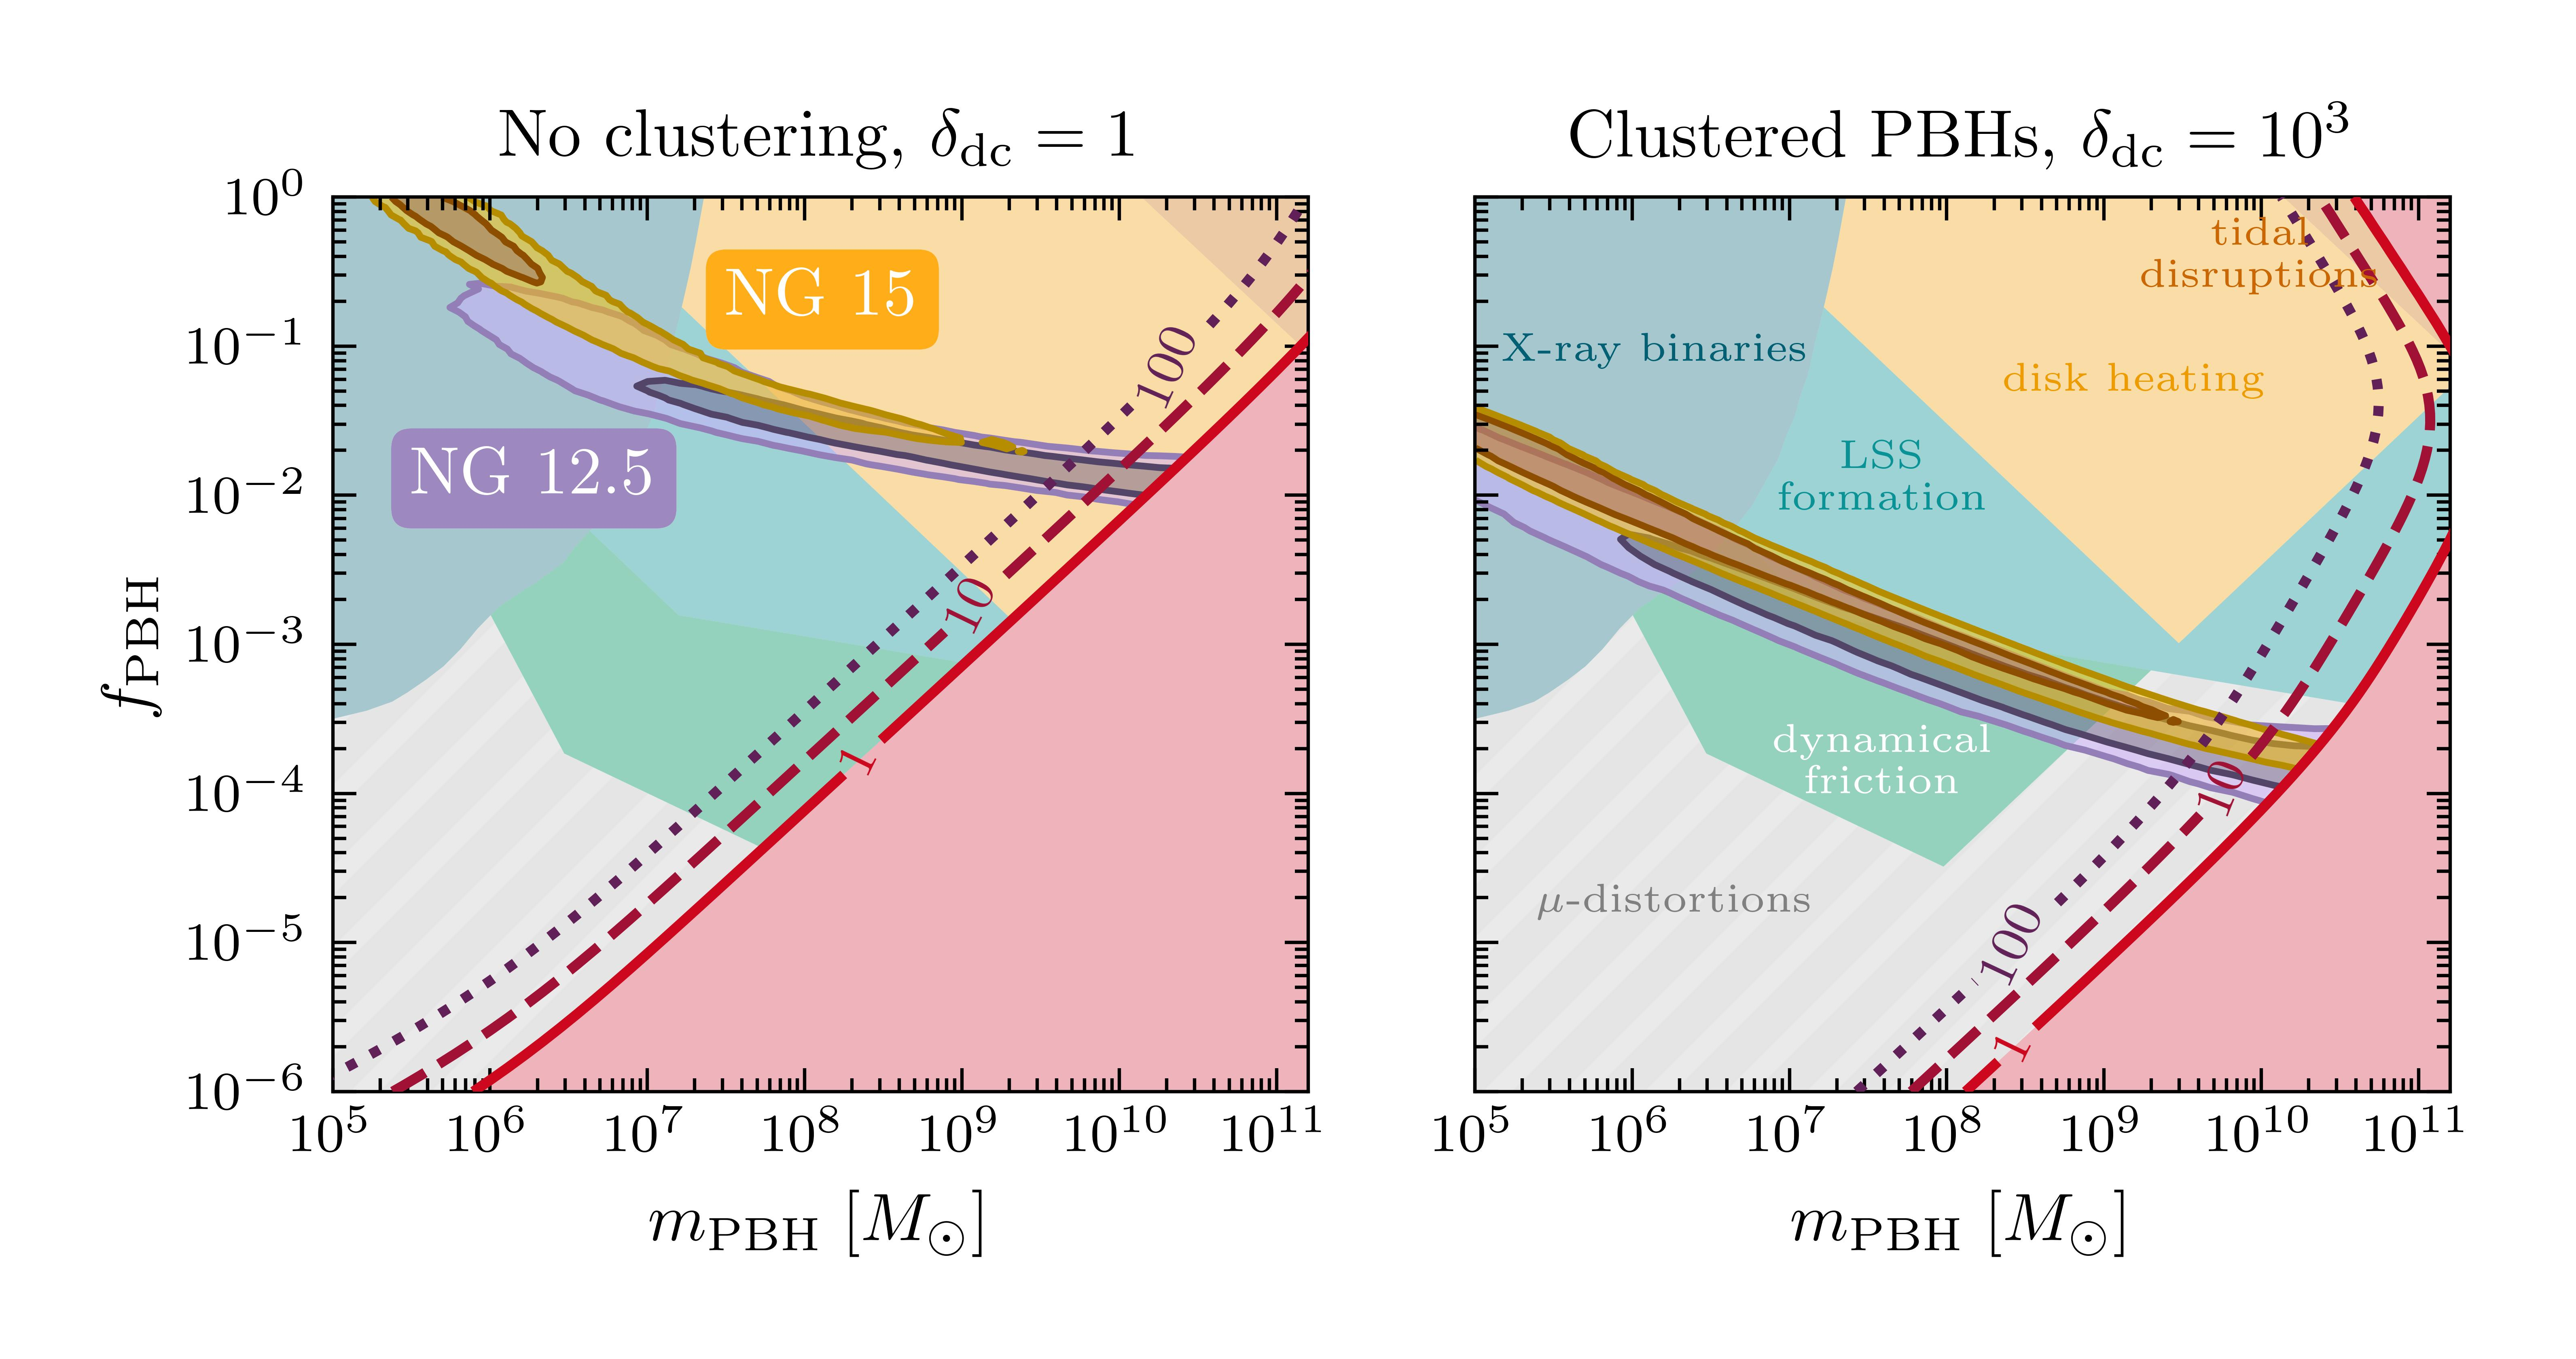
\includegraphics[width=\textwidth]{thesisplots/pbh/pbh_02_corrected.jpg}
	\caption{Best-fit regions where the \ac{NANOGrav} 15yr (orange) and 12.5yr (purple) data set can be explained by inspiraling \ac{PBH} binaries without clustering (left) and with significant clustering (right). We indicate regions, where $\bar{N} < 1$, $10$, and $100$ \ac{PBH} binaries are expected to contribute to the signal, and show complementary constraints as discussed in the main text.}
	\label{fig:res_explanation}
\end{figure}


In fig.~\ref{fig:res_explanation} we \graffito{Homogeneously distributed \acp{PBH} cannot explain the signal}  show the regions in \ac{PBH} mass $m_\pbh$ and DM fraction $f_\pbh$, where the \ac{NANOGrav} signal can be explained assuming merging \acp{PBH} with no clustering (left) and significant clustering with $\delta_\dc = 10^3$ (right). These contours are only expected to be reliable when the expected number of binaries is $\bar{N} \gtrsim 10$ (cf.~dashed dark red lines) as otherwise the signal  observable in \ac{NANOGrav} is expected to have significant deviations from the global average \ac{GWB} signal used in our analysis. Especially for $\bar{N} < 1$ (full red line) one would not even expect any \ac{GWB} signal in most realizations of \ac{PBH} binary distributions. These effects were neglected in~\cite{Atal:2020yic} that falsely concluded that the \ac{NANOGrav} signal could be explained in a region of parameter space without clustering, where $\bar{N} \lesssim 1$. We find that the case without clustering cannot explain the \ac{NANOGrav} signal once taking into account cosmological and astrophysical constraints.

Including clustering shifts the signal regions to smaller $f_\pbh$, enabling a consistent explanation of the \ac{PTA} data without violating observational constraints, provided that the \ac{PTA} formation \graffito{Clustering saves the explanation} mechanism does not result in significant $\mu$-distortions. Note that clustering is also expected to further open up parameter space for a consistent explanation as complementary constraints are expected to become weaker.

Comparing the results for the 15yr and 12.5yr data sets we note that the signal regions have shifted to larger $f_\pbh$, due to the preference for a larger \ac{GWB} in the new \graffito{15yr vs.~12.5yr data} data set~\cite{NANOGrav:2020bcs,NANOGrav:2023gor}, and there is a slight preference for lower masses, where the earlier emission of GWs leads to an increased slope, cf.~fig.~\ref{fig:rate_ogw}, as preferred by the new data~\cite{NANOGrav:2023gor}.

\begin{figure}[t]
	\centering
	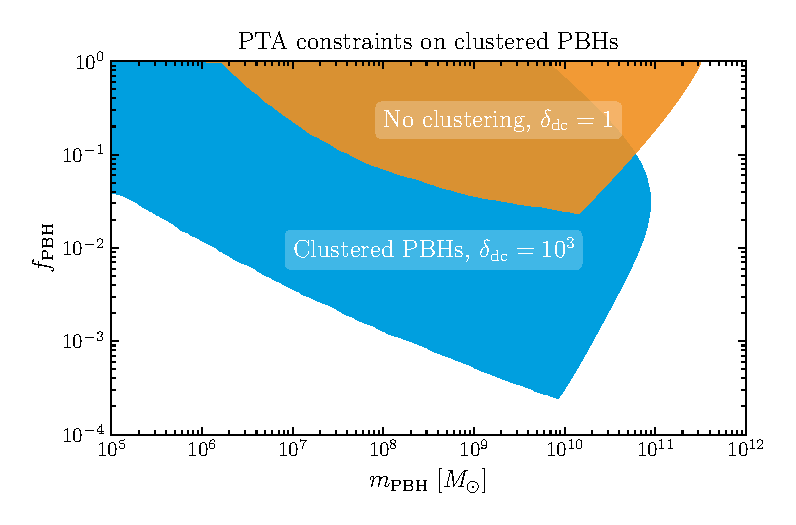
\includegraphics[width=\textwidth]{thesisplots/pbh/pbh_03}
	\caption{
		Constraints on \acp{PBH} from \ac{PTA} observations with no clustering (orange) and significant clustering $\delta_\dc = 10^3$ (blue). We conservatively cut the limits when the expected number of binaries contributing to the signal falls below $\bar{N} = 10$.}
	\label{fig:constraint}
\end{figure}

If the \ac{GWB} signal generated by inspiraling \ac{PBH} binaries becomes too large, above the regions \graffito{Novel \ac{PTA} constraints} explaining the \ac{PTA} data in fig.~\ref{fig:res_explanation}, the abundance of \acp{PBH} can be \emph{constrained} by \ac{PTA} observations. The constraints are shown in fig.~\ref{fig:constraint} with and without clustering, conservatively requiring $\bar{N} \geq 10$.

\section{Discussion and conclusions}
In this chapter we have studied the possibility that the signal observed by various \acp{PTA} is due to inspiraling primordial \acp{SMBHB}. If the \acp{PBH} are ``homogeneously'' distributed at their formation, i.e.~follow a Poisson distribution, significant cosmological and astrophysical constraints exclude the possibility of explaining the PTA signal with inspiraling \acp{PBH}. Instead considering a clustered spatial distribution of \acp{PBH} increases the binary merger rate and thus enables a \graffito{\acp{PTA} could have detected inspiral of clustered \ac{PBH}} consistent explanation of the \ac{PTA} signals with merging \ac{PBH} binaries. Crucially, we have checked that also the signal prediction is reliable in the relevant parameter space by computing the expected number of binaries contributing to the \ac{GW} signal. Further, we used \ac{PTA} data to constrain the \ac{PBH} parameter space when the \ac{GWB} generated during the inspiral would result in stronger signal strengths than the one detected.

The studied scenario may serve as a motivation for model builders to construct scenarios that can generate clustered supermassive \acp{PBH} without running into cosmological and astrophysical constraints, in particular due to $\mu$-distortions of the \ac{CMB} arising from \ac{PBH} formation.\graffito{Our model also features anisotropies} While the latest \ac{PTA} data finds no evidence for individual compact binary merger events on top of a stochastic background or anisotropies of the \ac{GW} spectrum, the situation might change in the future. Such a detection would likely invalidate most other cosmological explanations, while being a prediction of our scenario.

